\subsection{Kernel Density Estimation}
\label{sub:kernelDensityEstimation}

Finding a local crowd density can be a simple task. Simply define the local area, and count the number of people inside that areas, and divide it by the size of the local area. This process could then be repeated across multiple local areas, to give us the the local densities across the entire map. If the local areas are defined in a grid, we call this a histogram. While histograms provide a simple and fast way of estimating crowd densities, there are considerable drawbacks. The placement of the grid and your bin-width, which is the size of your grid cells, directly influences the end result~\cite{histogramDrawbacks}. This can give a skewed overview, and since we wish to avoid this, we need another approach.

Another method is to use kernel density estimation. With this approach we estimate the density continuously across the map. This is done by considering the density of any given point to be influenced according to the proximity of observations. We define this influence through a kernel function, which gives a probability distribution for each observation. By modifying the kernel function used in this approach it can be used to estimate the density of any the point on the map rather than probabilities of the observations. While this approach overcomes the drawbacks of histograms, it is considerably more complicated.

\subsubsection{Finding Local Crowd Densities}
There exists multiple kernel functions that can be used in the kernel density estimation. The most commonly used is the Gaussian distribution, also known as the normal distribution, given by the function in \cref{eq:1dGaussianDistribution}. The function, given the distance $d$ from an observation to the centre of the kernel, returns the probability of the observation. An observation in this context, is a sample drawn from the distribution. The Gaussian distribution is commonly used as a kernel function because it arises naturally, both in theory and in experiments.

\begin{equation}
\label{eq:1dGaussianDistribution}
K(d) = \frac{1}{\sqrt{2\pi}} e^{-\frac{1}{2} d^2}
\end{equation}

The plot of the function is shown in \cref{fig:1dGaussianDistributionPlot}. Notice that the function converges with the x axis in $-\infty$ and $\infty$. This means that if we were to use this function for calculating the local crowd density, we would have to consider every person in the data set, because the function is defined for every x value. For performance reasons, this is not preferable.

Another kernel function is the Epanechnikov kernel, given by the function in \cref{eq:1dEpanechnikovDistribution}.

\begin{equation}
\label{eq:1dEpanechnikovDistribution}
K(d) = \frac{3}{4} \left( 1-d^2 \right) \mathbbm{1}_{\{\left| d \right| \leq 1\}}
\end{equation}

Here $\mathbbm{1}_{\{|d| \leq 1\}}$ denotes the indicator function, meaning that if $|d|$ has a value less than or equal to 1, the function returns $1$, otherwise $0$. This means that any person placed outside this range in our data set can be ignored. This property can be seen in the plot of the function in \cref{fig:1dEpanechnikovDistributionPlot}, where one can also see that the function converges with the x axis at $-1$ and $1$.

\begin{figure}[htbp]
\begin{subfigure}[c]{.49\linewidth}
    \centering
    \begin{tikzpicture}[scale=0.9]
    \begin{axis}[
    axis y line=center,
    axis x line=middle,
    grid=both,
    xmin=-3,xmax=3,
    ymin=-0.2,ymax=1,
    xlabel=$x$,ylabel=$y$,
    x label style={at={(axis description cs:1,0.2)},anchor=east},
    y label style={at={(axis description cs:0.5,1)},anchor=north west},
    xtick={-3,-2,-1,0,1,2,3},
    ytick={-0.2,0,0.1,0.2,0.3,0.4,0.5,0.6,0.7,0.8,0.9,1},
    height=7.5cm,
    anchor=center]
    \addplot[mark=none, thick, samples=100, smooth] {gaussian2d(1)};
    \end{axis}
    \end{tikzpicture}
    \caption{Gaussion/normal distribution.}
    \label{fig:1dGaussianDistributionPlot}
\end{subfigure}
%
\begin{subfigure}[c]{.49\linewidth}
    \centering
    \begin{tikzpicture}[scale=0.9]
    \begin{axis}[
    axis y line=center,
    axis x line=middle,
    grid=both,
    xmin=-3,xmax=3,
    ymin=-0.2,ymax=1,
    xlabel=$x$,ylabel=$y$,
    x label style={at={(axis description cs:1,0.2)},anchor=east},
    y label style={at={(axis description cs:0.5,1)},anchor=north west},
    xtick={-3,-2,-1,0,1,2,3},
    ytick={-0.2,0,0.1,0.2,0.3,0.4,0.5,0.6,0.7,0.8,0.9,1},
    height=7.5cm,
    anchor=center]
    \addplot[mark=none, thick, samples=100, smooth, domain=-1:1] {epanechnikov2d(1)};
    \addplot[mark=none, thick, samples=100, smooth, domain=1:3] {0};
    \addplot[mark=none, thick, samples=100, smooth, domain=-1:-3] {0};
    \end{axis}
    \end{tikzpicture}
    \caption{Epanechnikov distribution.}
    \label{fig:1dEpanechnikovDistributionPlot}
\end{subfigure}
\caption{Kernel density function plots.}
\end{figure}

For a function to be a kernel function it must have an area of 1 beneath it and be symmetric around the y-axis. The actual choice of kernel function is of minor importance~\cite{masteropgave}, as long as it is a bell curve kernel function. The area of the Gaussian and Epanechnikov functions can be seen plotted in \cref{fig:1dGaussianEpanechnikovAreaPlot}. While both functions are bell curve kernel functions, Epanechnikov was chosen because of the indicator function, which makes the performance of an implementation faster. There are many other kernel functions that also apply the indicator function and has an area of 1 beneath its curve which could have been considered. However since the choice of the kernel function is of minor importance, we did not pursue other options.

\begin{figure}[htbp]
\begin{subfigure}[c]{.49\linewidth}
    \centering
    \begin{tikzpicture}[scale=0.9]
    \begin{axis}[
    axis y line=center,
    axis x line=middle,
    grid=both,
    xmin=-3,xmax=3,
    ymin=-0.2,ymax=1,
    xlabel=$x$,ylabel=$y$,
    x label style={at={(axis description cs:1,0.2)},anchor=east},
    y label style={at={(axis description cs:0.5,1)},anchor=north west},
    xtick={-3,-2,-1,0,1,2,3},
    ytick={-0.2,0,0.1,0.2,0.3,0.4,0.5,0.6,0.7,0.8,0.9,1},
    height=7.5cm,
    anchor=center]
    \addplot[mark=none, thick, samples=100, smooth] {gaussian2d(1)};
    \addplot[mark=none, thick, samples=100, smooth, fill=lightgray, fill opacity=0.5, restrict y to domain=0:1] {gaussian2d(1)};
    \end{axis}
    \end{tikzpicture}
    \caption{Gaussian/normal distribution.}
    \label{fig:1dGaussianAreaPlot}
\end{subfigure}
%
\begin{subfigure}[c]{.49\linewidth}
    \centering
    \begin{tikzpicture}[scale=0.9]
    \begin{axis}[
    axis y line=center,
    axis x line=middle,
    grid=both,
    xmin=-3,xmax=3,
    ymin=-0.2,ymax=1,
    xlabel=$x$,ylabel=$y$,
    x label style={at={(axis description cs:1,0.2)},anchor=east},
    y label style={at={(axis description cs:0.5,1)},anchor=north west},
    xtick={-3,-2,-1,0,1,2,3},
    ytick={-0.2,0,0.1,0.2,0.3,0.4,0.5,0.6,0.7,0.8,0.9,1},
    height=7.5cm,
    anchor=center]
    \addplot[mark=none, thick, samples=100, smooth, domain=-1:1] {epanechnikov2d(1)};
    \addplot[mark=none, thick, samples=100, smooth, domain=1:3] {0};
    \addplot[mark=none, thick, samples=100, smooth, domain=-1:-3] {0};
    \addplot[mark=none, thick, samples=100, smooth, fill=lightgray, fill opacity=0.5, domain=-1:1] {epanechnikov2d(1)};
    \end{axis}
    \end{tikzpicture}
    \caption{Epanechnikov distribution.}
    \label{fig:1dEpanechnikovAreaPlot}
\end{subfigure}
\caption{The area beneath both Epanechnikov and the Gaussian distribution.}
\label{fig:1dGaussianEpanechnikovAreaPlot}
\end{figure}

A kernel density estimation is performed for a specific point, and can be calculated as either absolute, relative, or probabilistic density. The absolute density is the amount of people per local crowd density point. This means that the densities for all points have to sum up to the total amount of people.

The relative densities are the absolute densities divided by the area that each point covers, for instance people per square meter. Since we want to be able to compare the values calculated for the crowd factors with certain limits, this is the type of kernel density we want to calculate.

The last kernel density type is probabilistic. This is the absolute densities divided by the total amount of people, meaning that the total sum of probabilistic local crowd densities has to be 1.

\subsubsection{Bandwidth}

Kernel functions denote the probability of finding an observation at certain distances from the kernel center. In our case, the probability denotes how much an observed person weighs for the density of the point. For our chosen kernel function, Epanechnikov, this ranges between between -1 and 1. 
This constant range presents a problem, since we do not know how far away observations affect the density. Therefore we want a way to adjust the limit marking which observations should be considered in the estimation.

This is done using a bandwidth variable. The Epanechnikov function with the bandwidth can be seen in \cref{eq:1dEpanechnikovDistributionWithH} and the plot of the function with a bandwidth of 5 is shown in \cref{fig:1dEpanechnikovDistributionWithHPlot}. The area of this function is still 1 and therefore holds the property of a \sinote*{kernel function?}{kernel density function}.

\begin{equation}
\label{eq:1dEpanechnikovDistributionWithH}
K(d) = \frac{3}{4 h} \left( 1-\left(\frac{d}{h}\right)^2 \right) \mathbbm{1}_{\left\{\left|\left(\frac{d}{h}\right)\right| \leq 1\right\}}
\end{equation}

Here $d$ is the distance from the center of the kernel function to the observation, and $h$ is the bandwidth.

\begin{figure}[htbp]
\centering
\begin{tikzpicture}[baseline]
\begin{axis}[
axis y line=center,
axis x line=middle,
grid=both,
xmin=-6,xmax=6,
ymin=-0.2,ymax=1,
xlabel=$x$,ylabel=$y$,
x label style={at={(axis description cs:1,0.2)},anchor=east},
y label style={at={(axis description cs:0.5,1)},anchor=north west},
xtick={-5,...,5},
ytick={-0.2,-0.1,0,0.1,0.2,0.3,0.4,0.5,0.6,0.7,0.8,0.9,1},
width=10cm,
height=7.5cm,
anchor=center]
\addplot[mark=none, thick, samples=100, smooth, domain=-6:-5] {0};
\addplot[mark=none, thick, samples=100, smooth, domain=5:6] {0};
\addplot[mark=none, thick, samples=100, smooth, fill=lightgray, fill opacity=0.5, domain=-5:5] {epanechnikov2d(5)};
\end{axis}
\end{tikzpicture}
\caption{The area beneath the Epanechnikov function with bandwidth 5.}
\label{fig:1dEpanechnikovDistributionWithHPlot}
\end{figure}

\subsubsection{Multidimensional Estimation}

So far we have only been looking at the distribution in one dimension. In our domain we get observations from a plane, giving us two dimensions to consider. This would require us to model our bandwidth as dependent on two variables, but given our domain we can instead extend the kernel function to work by calculating the distance from the kernel center to the observation, and therefore use a single variable bandwidth. This can be seen plotted in \cref{fig:3dEpanechnikov}.

\begin{figure}[htbp]
\centering
    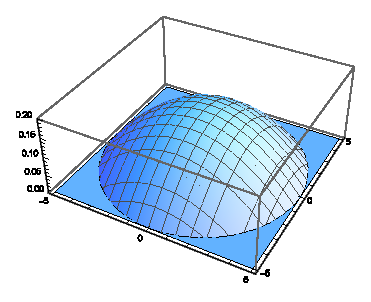
\includegraphics[width=0.5\textwidth]{3dEpanechnikov.eps}
    \caption{Epanechnikov over an area shown in 3 dimensions.}
    \label{fig:3dEpanechnikov}
\end{figure}

\Cref{fig:3dEpanechnikov} represents the distribution over a 2 dimensional space, where the third dimension represents how much the 2 dimensional points weights.

\subsubsection{Relative Density Form}

As explained earlier, the function is currently on a probability form, and not on the desired relative density form. In order to modify it, we first transform it to an absolute form. We assume that every person contributes the same density, so the mean value of the function should be 1. In order to \enquote{raise} the function so the mean value is 1, we can divide by the volume beneath the plane and multiply with the desired volume. The desired volume is that of which the kernel function has a mean value of 1. We start by calculating the current volume beneath the plane. This can be done through a triple integration on the function using a cylindrical coordinate set. As defined previously, the distance from point to center is the radius. The integration is done as shown in \cref{eq:volumeUnder3dEpanechnikov}.

\begin{equation}
\label{eq:volumeUnder3dEpanechnikov}
\int_0^{2 \pi} \int_0^h \int_0^1 \frac{3}{4 h} \left(1 - \left(\frac{r}{h}\right)^2\right) r \mathrm{ d}z\ \mathrm{d}r\ \mathrm{d}\theta\ = \frac{3 \pi h}{8}
\end{equation}

Because we are working in a cylindrical coordinate system, we use three variables to index every point in the coordinate system. $z$ is the height in the cylindrical system. $r$ is the distance from the center of the coordinate system to the point. $\theta$ is the angle in the coordinate system.

We now need to find the desired volume. Since we want a mean height to be 1, the area beneath the desired function is the same as a cylinder spanning over the same area with a height of 1. This cylinder has the volume of $h^2 \cdot \pi$ where $h$ is the bandwidth. To find the absolute densities we therefore divide by the actual volume and multiply by the desired volume, as shown in \cref{eq:absoluteDensitiesEpanechnikov}.

\begin{equation}
\label{eq:absoluteDensitiesEpanechnikov}
\frac{\frac{3}{4 h} \left(1 - \left(\frac{d}{h}\right)^2\right) \cdot \mathbbm{1}_{\left\{\left|\left(\frac{d}{h}\right)\right| \leq 1\right\}}}{\frac{3\pi h}{8}} \cdot \left(h^2 \cdot \pi\right)
\end{equation}

We here return to denoting the distance to the observation by $d$. To go from this absolute density form to a relative density form, we divide by the area of the absolute density form, which is $h^2 \cdot \pi$. The relative density can then be found as shown by the reduction in \cref{eq:relativeDensitiesEpanechnikov}.

\begin{equation}
\label{eq:relativeDensitiesEpanechnikov}
\begin{split}
&\frac{\frac{3}{4 h} \left(1 - \left(\frac{d}{h}\right)^2\right) \cdot \mathbbm{1}_{\left\{\left|\left(\frac{d}{h}\right)\right| \leq 1\right\}}}{\frac{3 \pi h}{8}} \cdot \frac{h^2 \cdot \pi}{h^2 \cdot \pi}\\
= &\frac{\frac{3}{4 h} \left(1 - \left(\frac{d}{h}\right)^2\right) \cdot \mathbbm{1}_{\left\{\left|\left(\frac{d}{h}\right)\right| \leq 1\right\}}}{\frac{3 \pi h}{8}}\\
= &\frac{2}{\pi \cdot h^2} \cdot \left(1-\left(\frac{d}{h}\right)^2\right) \cdot \mathbbm{1}_{\left\{\left|\left(\frac{d}{h}\right)\right| \leq 1\right\}}
\end{split}
\end{equation}

Finally, we sum the relative densities for all people, in order to find the estimated kernel density.

\begin{equation}
\label{eq:sumRelativeDensitiesEpanechnikov}
\frac{2}{\pi \cdot h^2} \cdot \sum_{i=1}^N \left(1-\left(\frac{d_{x,i}}{h}\right)^2 \cdot \mathbbm{1}_{\left\{\left|\left(\frac{d}{h}\right)\right| \leq 1\right\}}\right)
\end{equation}

Here $d_{x,i}$ is the distance from the desired point $x$ to the person $i$, and $N$ is the total amount of people. Since we have used a kernel function with an indicator function, in practice we only have to sum up densities for people within this of the point. This, as already mentioned, gives us some advantageous properties when we later in this chapter have to implement this function.

We can add some flexibility to \cref{eq:sumRelativeDensitiesEpanechnikov} by introducing an intensity variable $I$. See \cref{eq:sumRelativeDensitiesEpanechnikovWithIntensityWeight}. This variable will be utilised later in this section.

\begin{equation}
\label{eq:sumRelativeDensitiesEpanechnikovWithIntensityWeight}
\frac{2}{\pi \cdot h^2} \cdot \sum_{i=1}^N I \cdot \left(1-\left(\frac{d_{x,i}}{h}\right)^2 \cdot \mathbbm{1}_{\left\{\left|\left(\frac{d}{h}\right)\right| \leq 1\right\}}\right)
\end{equation}

%\includemovie[
%	poster,
%	toolbar, %same as `controls'
%	label=3depblabla.u3d,
%	text=(3depblabla.u3d),
%	3Daac=60.000000, 3Droll=0.000000, 3Dc2c=-0.000035 -3.301000 0.000000, 3Droo=3.301000, 3Dcoo=-0.000035 0.375017 0.000000,
%	3Dlights=CAD,
%]{\linewidth}{\linewidth}{figures/3depblabla.u3d}


%\pgfplotsset{width=7cm,compat=1.13}
%\usepgfplotslibrary{patchplots}
%\begin{tikzpicture}
%\begin{axis}[
%xmin=-5,xmax=5,
%ymin=-5,ymax=5,
%zmin=-0.2,zmax=0.2,
%xlabel=$x$,ylabel=$y$,ylabel=$z$]
%\addplot3[surf, patch type=rectangle, samples=40, restrict z to domain=-0.2:0] {epanechnikov3d(5)};
%addplot3[surf] {0};
%\addplot3[surf, patch type=rectangle, samples=40, restrict z to domain=0:0.2] {epanechnikov3d(5)};
%\end{axis}
%\end{tikzpicture}